\section*{RINEX Version 3.00 Library Enhancements}

The substantial changes between RINEX Version 3.00 (herein note R3)
and RINEX Version 2 (R2) resulted in the consideration of several
upgrade paths for implementation. The major design considerations for
discriminating advantages and disadvantages between choices were as
follows.
%
\begin{itemize}
  \item Full and straightforward backwards compatibility.
  \item Ease of testing.
  \item Minimal modifications required across the remainder of the
toolkit to integrate the new features.
\end{itemize}
%

Ultimately the choice was made to create an independent set of R3
classes with distinct names, simultaneously branching the GPSTk within
its Subversion repository.  This choice allows backwards compatibility
with R2, and allows for separate known versions for comparison testing
of R3 versus R2.
%
\begin{figure*}
   \centering
   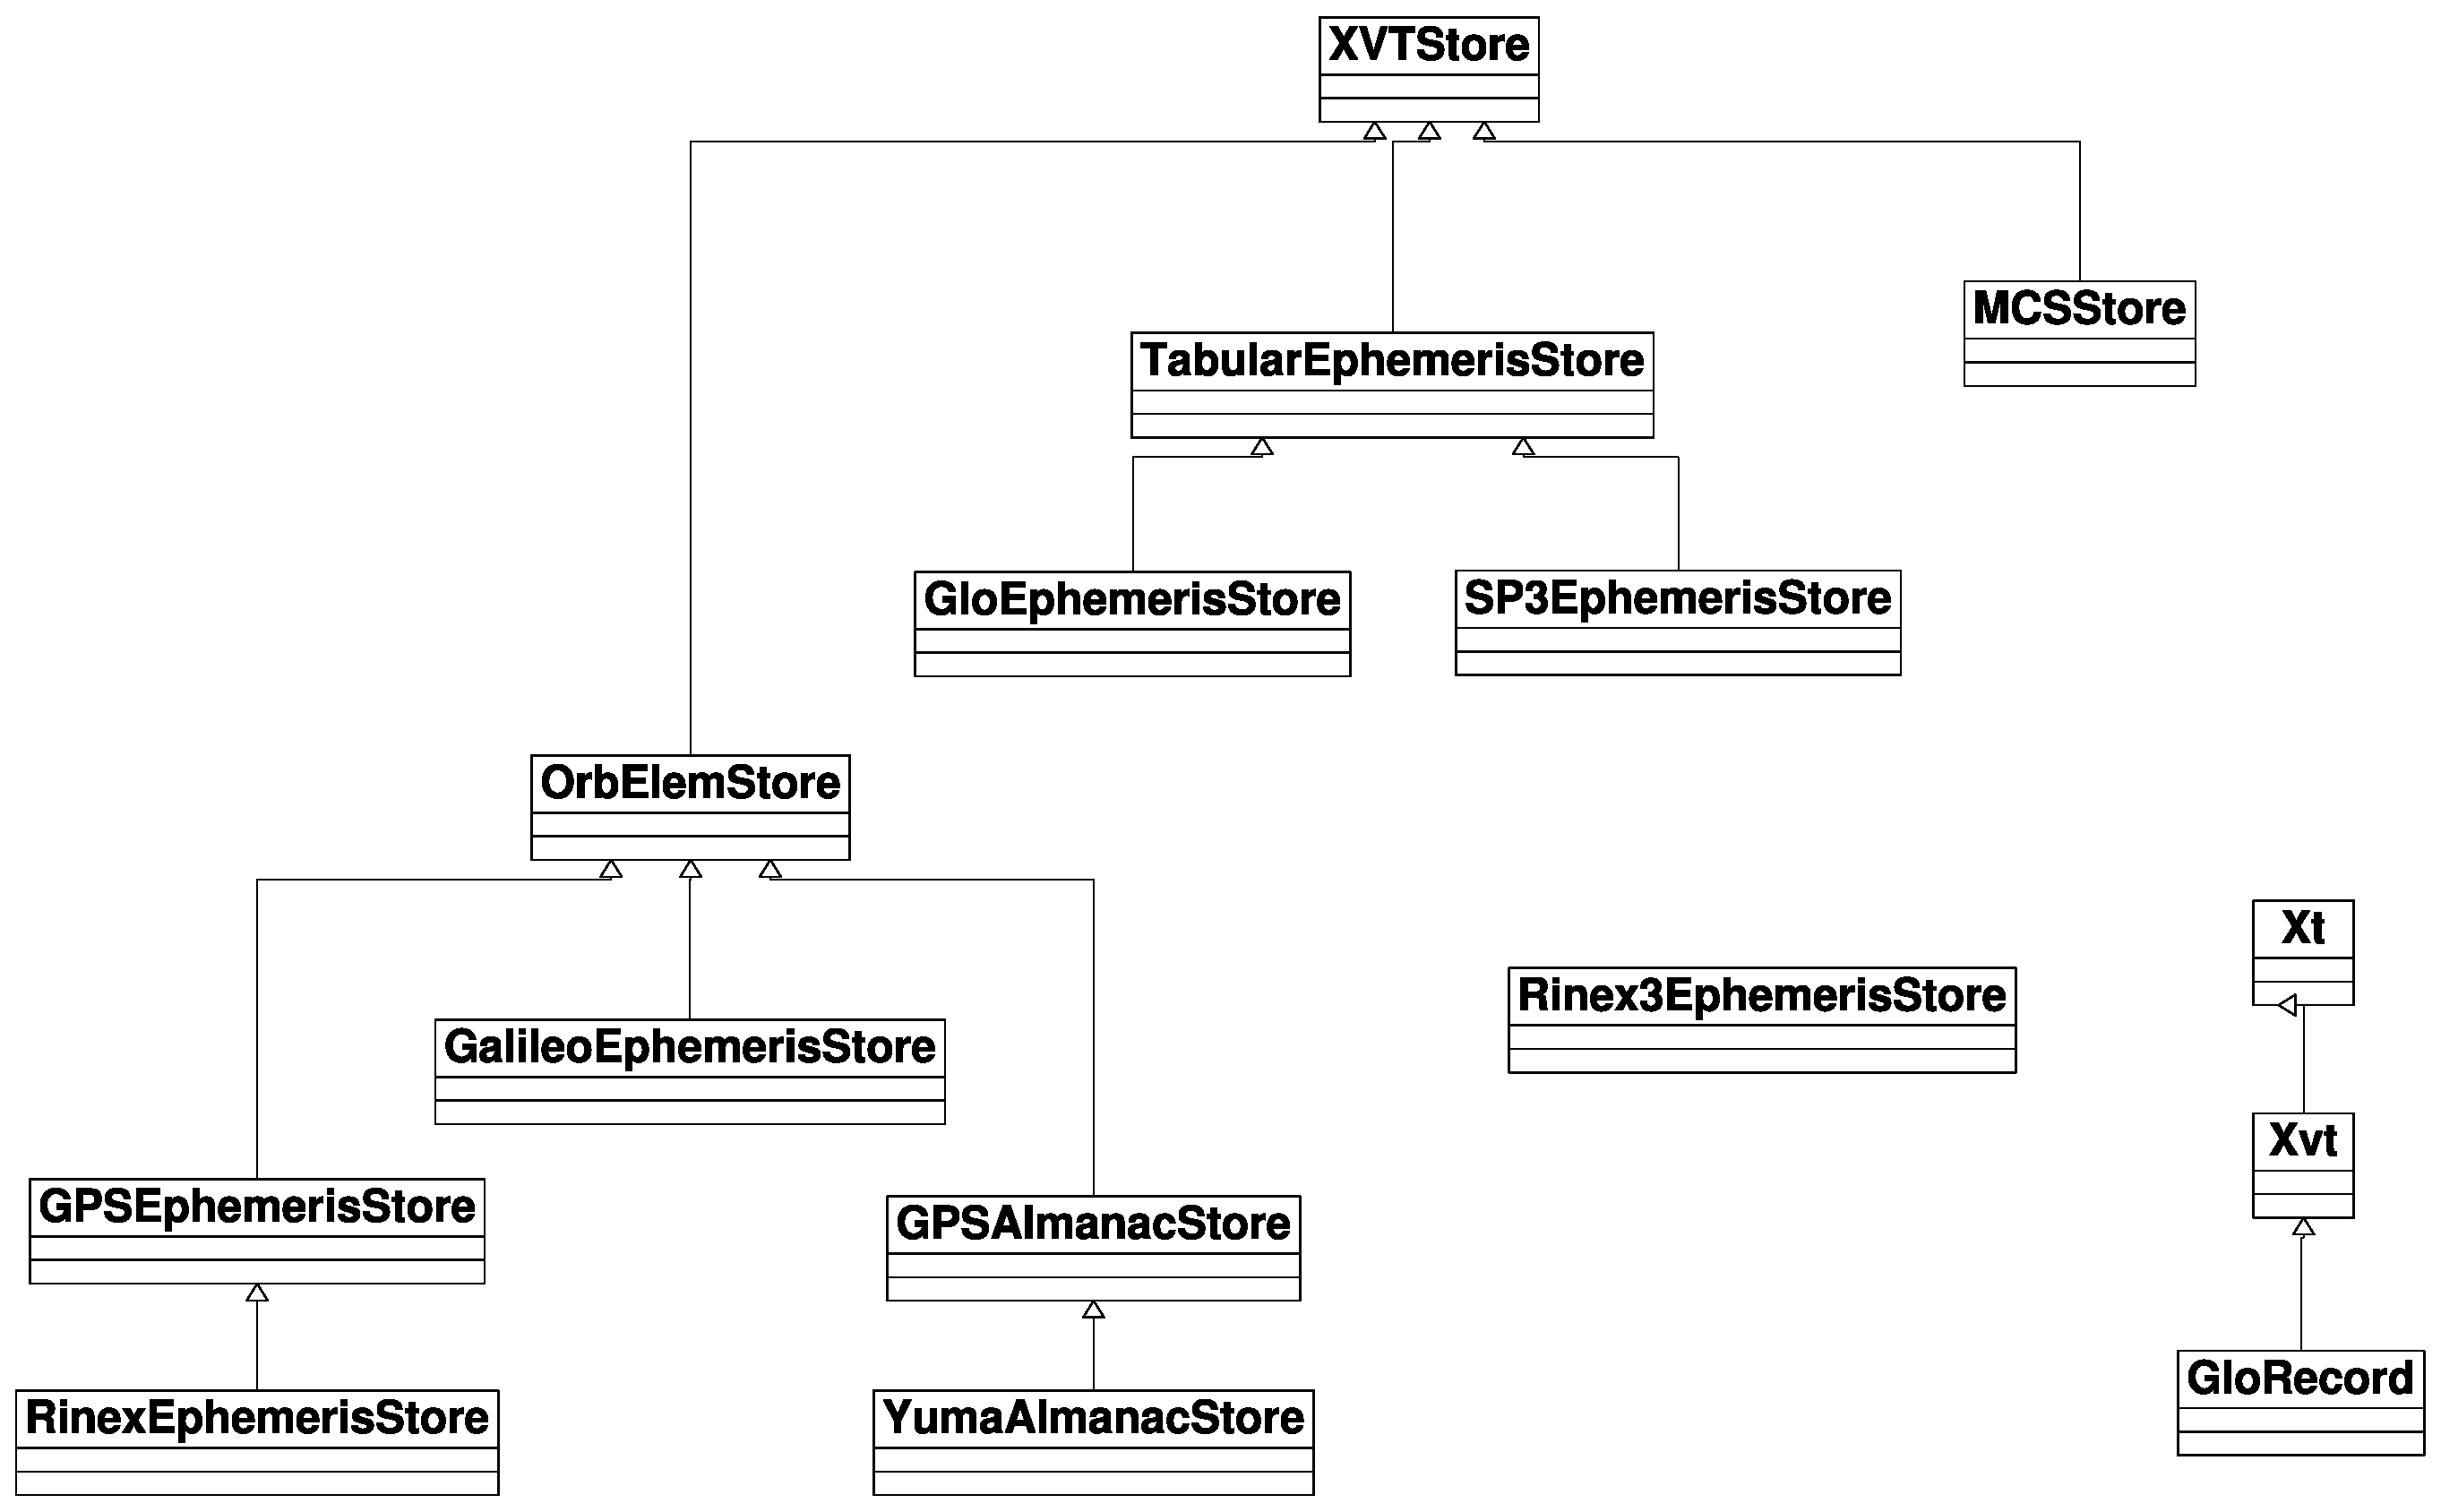
\includegraphics[width=5.5in,bb=79 313 1369 1107]{UML0709.eps}
   \caption{Unified Modeling Language (UML) diagram showing inheritance relationships among RINEX Version 3.00 classes.}
   \label{fig:rinex3}
\end{figure*}
%
Figure~\ref{fig:rinex3} depicts the class structure introduced to
support R3 capabilities.

%-------------------------------------------------------------------------------
\subsection*{Time System}

The GPSTk originally assumed that all times are given in the GPS time
system.  Since this is not true in a multi-GNSS world, a Time System
(TS) data structure was added to keep track of what time frame epochs
are actually reported in. The R3 standard specifies that epoch data
for a given GNSS be given in that GNSS's native time system.  As a
result, the GPSTk has been designed to automatically encode the TS
data structure along with the observations.

%-------------------------------------------------------------------------------
\subsection*{Coordinate System}

In the same vein, each GNSS uses its own realization of the
International Terrestrial Reference Frame (ITRF) as its coordinate
system.  For GPS this is WGS84(G1150), while for GLONASS it is PZ-90.
Galileo will use the Galileo Terrestrial Reference System (GTRF).
Japan's QZSS will use JGS, which differs from the GTRF by less than
2~cm.  The disagreement between different systems varies in general,
but the agreed-upon realization goal is 2-3~cm in the near future.

We have added support for the standard reference frames to the GPSTk,
as well as the ability to transform data between reference frames via
a Helmert transformation~\cite{Hofmann2008}, defined by
%
\begin{equation*}
{\bf X}_{A} = {\bf a} + \mu {\bf R} {\bf X}_{B}.
\end{equation*}
%
in which $\bf X$ denotes a position vector as a column matrix, $A$ and $B$ denote reference frames, $\mu$ is a scale factor and ${\bf a}$ is an offset or bias.

%-------------------------------------------------------------------------------

\subsection*{Data Storage and Access}

Observation, navigation, and meteorological data have to be stored for
access (there are only those three data types in R3).  This data
storage should be efficient.  The current implementation of R2
handling uses a ``map of maps'' (MoM) approach \cite{Stroustrup2000}.
In this approach, the actual data is stored in instances of a data
element class, which become the values in a map keyed by epoch (time).
Instances of that map are then stored as values in another map, this
one keyed by satellite vehicle ID.  The advantage of this approach is
that this creates a poor-man's ``database'' that is easily accessible
by the most identifiable tag, time.  Other possible approaches include
filling matrices, valarrays, linked lists or possibly other data
types.

For R3, we choose to stay with the MoM design based on an assessment that  
the current implementation of data storage in R2 is
acceptable in usability and speed, as well as being quite flexible. However, there are 
some revisions.  For
example, each GNSS has its own MoM, belonging to its own storage
class.  A new class specific to reading R3 files contains an instance
of each possible GNSS MoM, and inserts new data into the appropriate
MoM as it is read in.  Look-ups can then be targeted to a specific
GNSS, or scanned over all MoMs, depending on the user's requirements.

%-------------------------------------------------------------------------------

\subsection*{Navigation Data}

R3 expanded the navigation broadcast message (``Nav'') data type to
include general GNSS Nav messages.  These formats can be quite
different. For example, Galileo's broadcast ephemerides format is
similar to GPS \cite{Hofmann2008}. However, GLONASS, the Space-based augmentation
system (SBAS), and QZSS, use tabular ephemerides \cite{glonassicd50}.  A major
restructuring of the GPSTk ephemeris processing classes was required in order to
be able to handle the R3 standard, though it currently includes only
GLONASS.

The data storage class was more cleanly split into two
branches.  One is the parent class for all tabular-type GNSSs
(GLONASS, QZSS), while the other is for those which broadcast orbital
element data (GPS, Galileo).  It should be noted that precise
ephemerides in SP3 files are presented in tabular format.  Thus, the
SP3 classes remain a subclass of \gpstkclass{TabularEphemerisStore}.  We remark here only that separate
naming for the R3 classes allowed us to keep the R2 classes in place,
and with invisible backwards compatibility.  That is, R2 users will
not have to change their existing applications to use the new GPSTk
library.

%-------------------------------------------------------------------------------

\subsection*{Observation Data}

Observation (``Obs'') data refers to any measurement of (pseudo)range,
phase, Doppler or other signal quantity made with a GNSS receiver.  R3
Obs data files have changed significantly, providing support for
additional data, e.g. moving receivers or antenna details, but there
were subtle, significant structural changes.  Chief among these is Obs
type code list and format.  Obs files may now include multiple GNSS
data in a file, which requires more detailed header information on
what data will is present for each GNSS.  There are new data
structures for satellite ID.  Epochs are presented differently.

The new R3 Obs classes in the GPSTk had to be significantly modified
to handle these changes.  Some of the data is stored in maps (and even
maps of maps) to simplify access over different GNSSs.  The extent of
changes in the R3 standard will require Obs data users to
significantly change the way they write their applications.  It has
always been up to the user to store Obs data once read in; we continue
to not provide any inherent Obs data storage classes (e.g. MoMs) in
this upgrade.

